\section{Алгоритм}
\subsection{Чтение и предварительный анализ данных}
Применяя метод \texttt{read\_csv} библиотеки \texttt{pandas}, формируем дата-фрейм:



\noindent
%---------------------------------------
%---------------------------------------
\SetTblrInner{rowsep=3pt}
%---------------------------------------
\begin{longtblr}
[
caption = {Исходные данные},
]	
{
colspec = {
X[r,f]
X[r,f,4] 
X[r,f,4] 
X[r,f,4] 
X[c,f,4]
X[r,f,4]
},
width = \linewidth,
rowhead = 1, 
rowfoot = 0,
row{odd} = {}, 
row{even} = {},
rows    = {font=\scriptsize},
row{1}  = {font=\scriptsize\bfseries}
}
&
Постоянные зрители 
& 
Новые зрители
&
Просмотры 
&
...
& 
Доля подписок
\\
\hline[1pt]

\textbf{0} & 41 & 11 & 114 & ... & Низкая 
\\
\hline
\textbf{1} & 29 & 5 & 79 & ... & Низкая 
\\
\hline
\textbf{2} & 54 & 47 & 84 & ... & Высокая 
\\
\hline
\textbf{...} & ...   & ...  & ... & ... & ... 
\\
\hline
\textbf{498} & 35 & 24 & 102 & ... & Низкая 
\\
\hline
\textbf{499} & 40 & 29 & 88 & ... & Низкая 
\\
\hline[1pt]
\end{longtblr}
%---------------------------------------

\noindent
При помощи метода \texttt{describe} библиотеки \texttt{pandas} выводим характеристики распределений числовых признаков:

\noindent
%---------------------------------------
%---------------------------------------
\SetTblrInner{rowsep=3pt}
%---------------------------------------
\begin{longtblr}
	[
	caption = {Исходные данные},
	]	
	{
		colspec = {
			X[r,m, 3]
			X[r,m] 
			X[r,m] 
			X[r,m] 
			X[r,m]
		},
		width = \linewidth,
		rowhead = 1, 
		rowfoot = 0,
		row{odd} = {}, 
		row{even} = {},
		rows    = {font=\scriptsize},
		row{1}  = {font=\scriptsize\bfseries}
	}
	&
	mean 
	& 
	std
	&
	min 
	&
	max

	\\
	\hline[1pt]
	
	\textbf{Постоянные зрители} & 3.942000 & 7.925419 & 0.0000 & 56.0000
	\\
	\hline
	\textbf{Новые зрители} & 32.586000 & 94.640204 & 0.0000 & 1100.0000
	\\
	\hline
	\textbf{Просмотры} & 100.530000 & 170.646446 & 5.0000 & 1880.0000 
	\\
	\hline
	\textbf{Клики по элементам конечной заставки} & 0.508000   & 1.048874  & 0.0000 & 9.0000 
	\\
	\hline
	\textbf{Показы элементов конечной заставки} & 58.786000 & 79.566260 & 0.0000 & 792.0000  
	\\
	\hline
	\textbf{Показы тизеров} & 3.942000 & 7.925419 & 0.0000 & 56.0000  
	\\
	\hline
	\textbf{Среднее число просмотров одним пользователем} & 1.241784 & 0.171804 & 1.0000 & 2.6000
	\\
	\hline
	\textbf{Уникальные зрители} & 79.674000 & 133.822347 & 3.0000 & 1465.0000
	\\
	\hline
	\textbf{Средний процент просмотра} & 35.109640 & 13.616501 & 9.5200 & 74.5700
	\\
	\hline
	\textbf{Отказались от подписки} & 0.010000 & 0.099598 & 0.0000 & 1.0000
	\\
	\hline
	\textbf{Новые подписчики} & 0.360000 & 1.000200 & 0.0000 & 9.0000
	\\
	\hline
	\textbf{Новые комментарии} &0.056000 & 0.254939 & 0.0000 & 2.0000
	\\
	\hline
	\textbf{Поделились} & 0.640000 & 1.811343 & 0.0000 & 17.0000
	\\
	\hline
	\textbf{Отметки 'Не нравится'} & 0.064000 & 0.322664 & 0.0000 & 4.0000
	\\
	\hline
	\textbf{Отметки 'Нравится'} & 1.486000 & 3.079085 & 0.0000 & 40.0000
	\\
	\hline
	\textbf{Время просмотра (часы)} & 4.023387 & 7.663491 & 0.3026 & 90.9871
	\\
	\hline
	\textbf{Показы} & 621.738000 & 797.378602 & 39.0000 & 8889.0000
	\\
	\hline
	\textbf{CTR для значков видео (\%)} & 5.969620 & 3.318488 & 0.0000 & 21.2400
	\\
	\hline[1pt]
\end{longtblr}
%---------------------------------------

\noindent
И характеристики распределения признака 'Доля подписок':

\noindent
%---------------------------------------
%---------------------------------------
\SetTblrInner{rowsep=3pt}
%---------------------------------------
\begin{longtblr}
	[
	caption = {Исходные данные},
	]	
	{
		colspec = {
			X[r,m, 3]
			X[r,m] 
			X[r,m] 
			X[r,m] 
		},
		width = \linewidth,
		rowhead = 1, 
		rowfoot = 0,
		row{odd} = {}, 
		row{even} = {},
		rows    = {font=\scriptsize},
		row{1}  = {font=\scriptsize\bfseries}
	}
	&
	unique 
	& 
	top
	&
	freq 
	
	\\
	\hline[1pt]
	
	\textbf{Доля подписок} & 2 & Низкая & 400
	\\

	\hline[1pt]
\end{longtblr}
%---------------------------------------

\noindent
Здесь \texttt{unique}~--- количество уникальных значений, \texttt{top}~--- значение, обладающее максимальной частотой (модальное значение), \texttt{freq}~--- частота модального значения.

Мы видим, что числовые признаки имеют сильно различающийся разброс (на несколько порядков), а имеющиеся два класса строкового признака 'Доля подписок' не сбалансированы (представлены в отношении 4:1). Отметим, что несбалансированность классов является одной из причин, по которой мы среди прочих выбрали именно метрику AUC: эта метрика оценивает качество разделения на классы вне зависимости от пропорций, в которых состоят условно положительный и условно отрицательный классы.

\subsection{Преобразование целевого признака\\ в числовой формат}

Целевая функция алгоритма классификации, который мы собираемся обучить и настроить~---  это признак 'Доля подписок', значения которого относятся к строковому типу: 'Низкая доля'/'Высокая доля'. Но алгоритмы классификации, в том числе и \texttt{KNeighborsClassifier} библиотеки \texttt{sklearn},  могут работать только с числовыми данными, а любая попытка применить классификатор к строковым записям приедет к сообщению об ошибке. Поэтому, прежде чем приступать к построению классификатора, нам нужно перевести строковые данные в числовой формат. 

Мы применяем метод \texttt{loc} библиотеки \texttt{pandas} и осуществляем  замену по условию в столбце 'Доля подписок', а именно: каждое строковое значение 'Низкая доля' мы заменяем нулем, а каждое значение 'Высокая доля'~--- единицей. Теперь все данные имеют числовой формат, причем, 18 признаков относятся к типу \texttt{float}, а  целевой признак 'Доля подписок'~--- к типу \texttt{int}, и он принимает значения 0 или 1.

\subsection{Разбиение данных на обучающую\\ и тестовую выборки}

Еще один предварительный шаг моделирования состоит в разбиении данных на обучающую и тестовую выборки, что является важнейшей практикой в машинном обучении. 
Следует отметить, что основная цель машинного обучения заключается в создании модели, которая может обобщать знания на новые, ранее не встречавшиеся данные. Разделение данных на обучающую и тестовую выборки позволяет оценить, насколько хорошо модель справляется с обобщением. Модель обучается на тренировочной выборке и затем тестируется на тестовой выборке. Если модель хорошо справляется с предсказанием на тестовой выборке, то это указывает на ее способность обобщать. В целом, разбиение данных на обучающую и тестовую выборки является необходимой практикой в машинном обучении для обеспечения надежной оценки модели и предотвращения переобучения.

Чтобы разбить данные на обучающую и тестовую выборки мы используем метод \texttt{train\_test\_spli}t из модуля \texttt{model\_selection} библиотеки \texttt{sklearn}. Мы разбиваем данные в пропорции 8:2, при этом 80\% записей приписываем к обучающей выборке, а оставшиеся 20\%~--- к тестовой выборке.

\subsection{Построение и обучение модели\\ классификации}

Формируем объект \texttt{model}, относящийся к классу \texttt{KNeighborsClassifier}, используя в качестве параметра модели 20 ближайших соседей, после чего, применяя к объекту \texttt{model} метод \texttt{fit}, обучаем модель на обучающей выборке, используя в качестве разметки значения признака 'Доля подписок'.


\subsection{Прогноз на основе обученной модели}

Классификатор \texttt{KNeighborsClassifier} способен возвращать два типа прогноза при помощи методов \texttt{predict} и \texttt{predict\_proba}. А именно:

\medskip

\begin{itemize}
	\item метод \texttt{predict} получает на вход объекты тестовой выборки и возвращает предсказанные метки классов, то есть 0 или 1, в зависимости от того, какой класс оказался в большинстве среди k ближайших соседей каждого из объектов;
	\item метод \texttt{predict\_proba} тоже получает на вход объекты тестовой выборки, но возвращает не метки классов, а вероятности $p_0$ и $p_1$, где $p_0$ означает вероятность принадлежности объекта к классу 0, а $p_1$~--- к классу 1.
\end{itemize}

\medskip
\noindent
Нам требуется именно вероятностный прогноз принадлежности к классу~1. Поэтому в качестве прогнозируемых значений классификатора далее мы будем использовать массив вероятностей, и, поскольку метод \texttt{predict\_proba} возвращает двумерный массив с двумя вероятностями, мы специально указываем, что в качестве рабочих вероятностей мы будем использовать тот столбец возвращаемого двумерного массива, который соответствует положительному классу.

\subsection{ Построение ROC-кривой}
Для построения ROC-кривой мы применяем метод \texttt{roc\_curve} из модуля \texttt{metrics} библиотеки \texttt{sklearn}. Этот метод возвращает три массива:
\medskip


\begin{enumerate}
	\item массив p, который содержит все возникающие в классификаторе пороги бинаризации;
	\item массив FPR, который содержит соответствующие порогам бинаризации величины False Positive Rate (подробнее о величине FPR см. [2]);
	\item массив TPR, который содержит соответствующие порогам бинаризации величины True Positive Rate (подробнее см. [2]).
\end{enumerate}

\medskip

Затем при помощи модуля \texttt{pyplot} библиотеки \texttt{matplotlib}, строим ROC-кривую, используя массивы FPR и TPR, как горизонтальную и вертикальную переменные соответственно. Кроме того, мы используем метод \texttt{roc\_auc\_score} из модуля \texttt{metrics} библиотеки \texttt{sklearn}, который возвращает площадь под ROC-кривой, то есть, значение метрики AUC, и получаем кривую вместе с указанием ее меры (см. рис.~1(a)).


\begin{figure}[!htb]
	\centering
	\begin{minipage}{0.32\textwidth}
		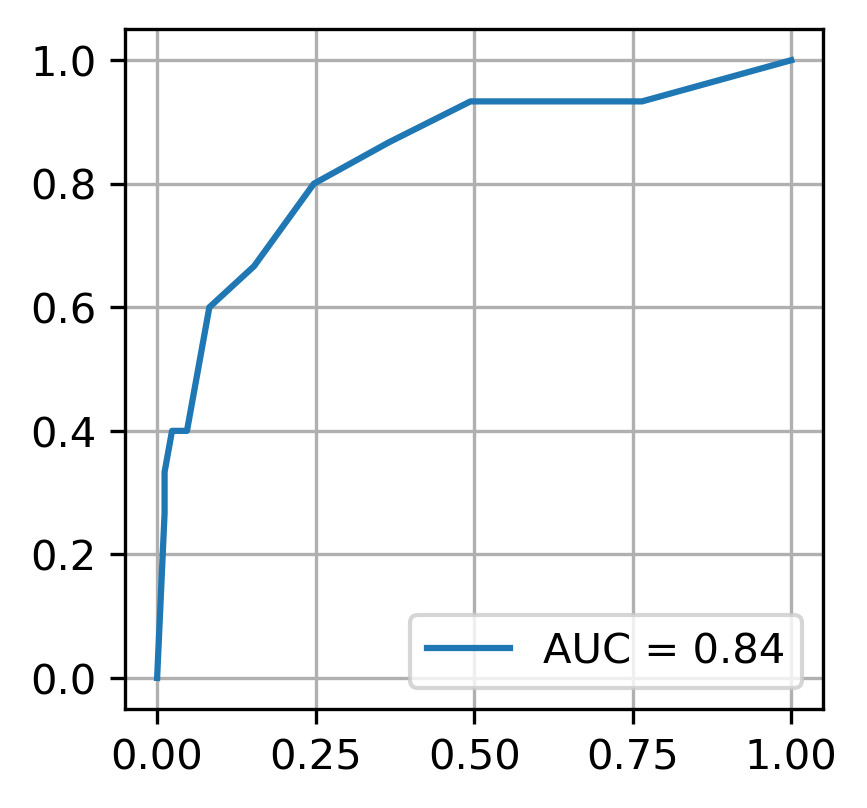
\includegraphics[width=\linewidth]{pictures/ROC-кривая}
	\end{minipage}
	\hspace{0.1\textwidth}
	\begin{minipage}{0.32\textwidth}
		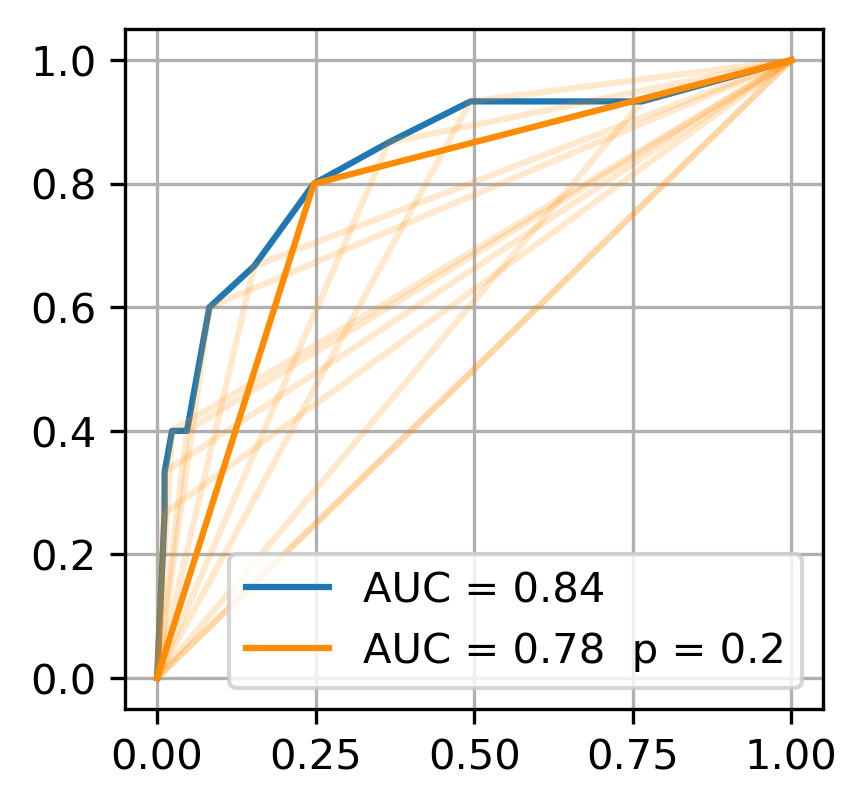
\includegraphics[width=\linewidth]{pictures/Прогон порогов бинаризации}

	\end{minipage}
	\caption{ROC-кривая (a) и подбор порога бинаризации (b)}
\end{figure}


\subsection{Вычисление оптимального порога\\ бинаризации}

В случае бинарного прогноза ROC-кривая представляет собой ломаную линию из двух звеньев, которая характеризуется единственной точкой внутри единичного квадрата, а метрика AUC вычисляется как площадь под этой линией. То есть для каждого порога бинаризации получается своя бинарная ROC-кривая со своим значением метрики AUC. Запуская цикл по всем значениям из массива p, получаем серию таких характеристик и выбираем тот порог бинаризации, который отвечает максимальному значению метрики AUC (см. рис.~1(b)).

\subsection{Повторный запуск}
Напомним, что прежде чем начинать исследование, мы произвели случайное разбиение набора данных на обучающую и тестовую выборки. Эффект случайности неизбежно проявится, если мы заново разобьём данные: возникнут новые соотношения между представителями классов (особенно, если учесть, что классы не сбалансированы), получатся какие-то другие значения метрики AUC и порога бинаризации $p$. 

\begin{figure}[!htb]
	\centering
	\begin{minipage}{0.32\textwidth}
		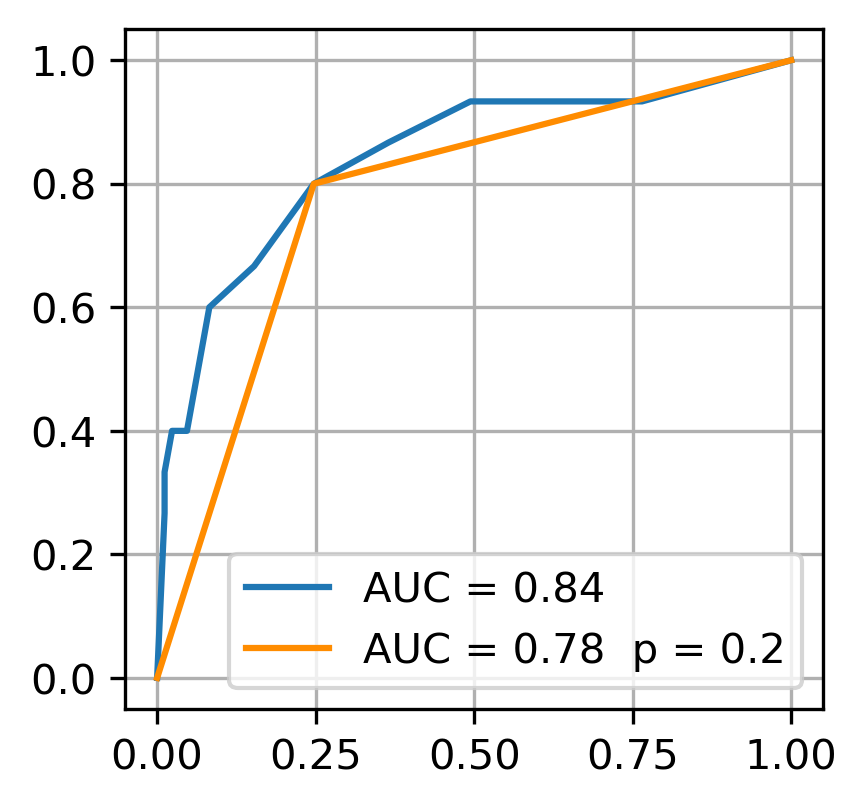
\includegraphics[width=\linewidth]{pictures/Первый запуск}
	\end{minipage}
	\hspace{0.1\textwidth}
	\begin{minipage}{0.32\textwidth}
		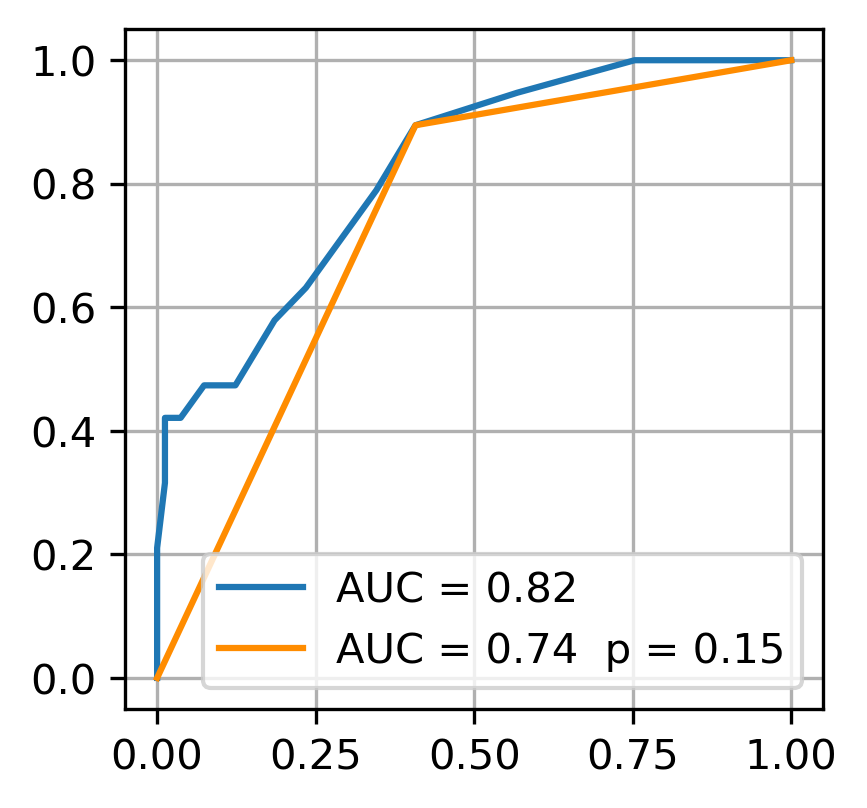
\includegraphics[width=\linewidth]{pictures/Повторный запуск}
		
	\end{minipage}
	\caption{Первый (a) и повторный (b) запуски}
\end{figure}
\noindent
Мы производим повторный запуск алгоритма и при новом случайном разбиении действительно получаем другой результат (см. рис.~2(b)).
Мы видим, что при повторном запуске порог бинаризации принимает значение 0.15, а не 0.2, как это было первоначально, и кроме того, не приводя подробных иллюстраций, просто отметим, что при следующих повторных запусках порог бинаризации варьируется случайным образом в широком диапазоне от 0.1 до 0.35.

\subsection{Усреднение ROC-кривой на множестве\\запусков}
Чтобы избежать эффекта случайности, производим 250 запусков и усредняем все возникающие при каждом запуске характеристики (см. рис.~3):
\medskip
\begin{enumerate}
	\item ROC-кривую,
	\item метрику AUC для вероятностного прогноза,
	\item ROC-кривую, получающуюся в результате оптимальной бинаризации,
	\item метрику AUC для бинарного прогноза,
	\item порог вероятности $p$, на котором происходит оптимальная бинаризация.
\end{enumerate}
\medskip
\begin{figure}[!htb]
	\centering
	\begin{minipage}{0.32\textwidth}
		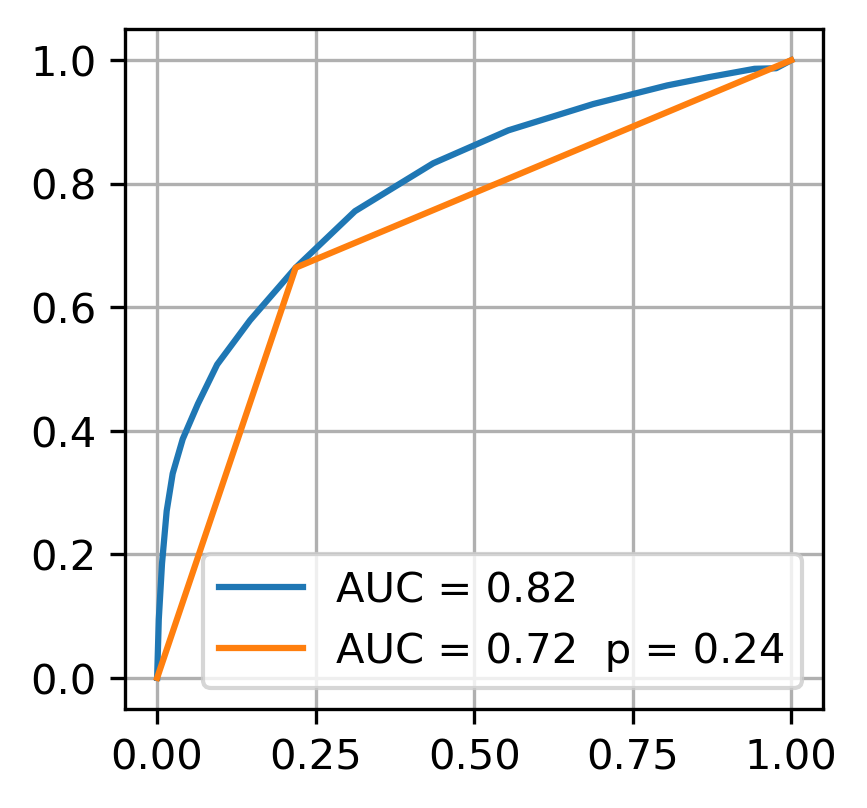
\includegraphics[width=\linewidth]{pictures/Усредненная бинаризация}
	\end{minipage}
	\caption{Усреднение на множестве запусков}
\end{figure}
\medskip
\noindent
После этого в результате усреднения порог бинаризации стабилизируется примерно на уровне $p=0.24$.

\subsection{Сравнение оптимизированного прогноза\\ с дефолтным}

Теперь у нас есть возможность сравнить прогноз, который получается после оптимальной бинаризации вероятностей, с дефолтным прогнозом, который получается прямым голосованием ближайших соседей. 
Мы сравниваем по метрике AUC оптимизированный прогноз с дефолтным прогнозом метода \texttt{predict} классификатора \texttt{KNeighborsClassifier}, по следующей схеме:
\medskip
\begin{enumerate}
	\item запускаем случайное разбиение данных на обучающую и тестовую выборки;
	\item вызываем метод \texttt{predict} и получаем дефолтный бинарный прогноз;
	\item вызываем метод \texttt{predict\_proba} и получаем вероятностный прогноз;
	\item находим порог бинаризации вероятностного прогноза, который отвечает максимальному значению метрики AUC , так же, как это делалось на шаге 3.8;
	\item выполняем бинаризацию вероятностного прогноза на найденном пороге;
	\item пользуясь методом \texttt{auc\_score}, находим значения метрики AUC для дефолтного и бинаризированного прогнозов;
	\item  строим все ROC-кривые, отмечаем все метрики AUC и выводим порог бинаризации p (см. рис. 4 (a)).

\end{enumerate}
\medskip

Мы видим, что метрика AUC для вероятностного прогноза (синяя линия) равна 0.81. Для бинарного прогноза, который получается после бинаризации вероятностного (желтая линия), метрика AUC равна 0.78. При этом оптимальный порог бинаризации $p = 0.15$. Для дефолтного бинарного прогноза (желтая пунктирная линия) метрика AUC равна 0.62. Затем производим повторный запуск при новом случайном разбиении данных на обучающую и тестовую выборки (см. рис. 4 (b)).

\begin{figure}[!htb]
	\centering
	\begin{minipage}{0.32\textwidth}
		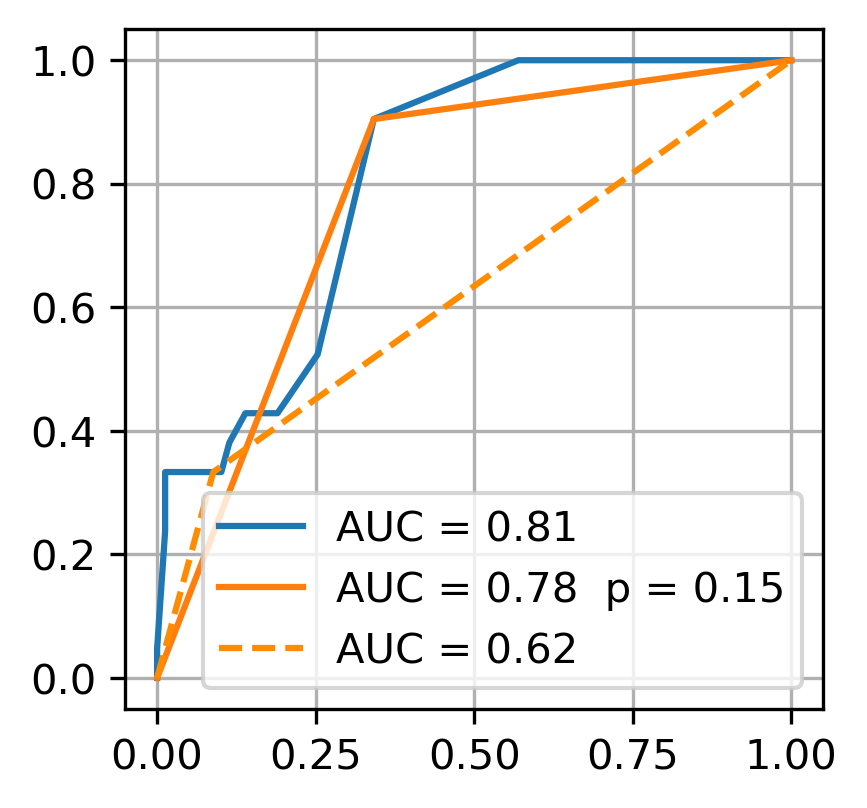
\includegraphics[width=\linewidth]{pictures/Обе метрики при 0 запуске}
	\end{minipage}
	\hspace{0.1\textwidth}
	\begin{minipage}{0.32\textwidth}
		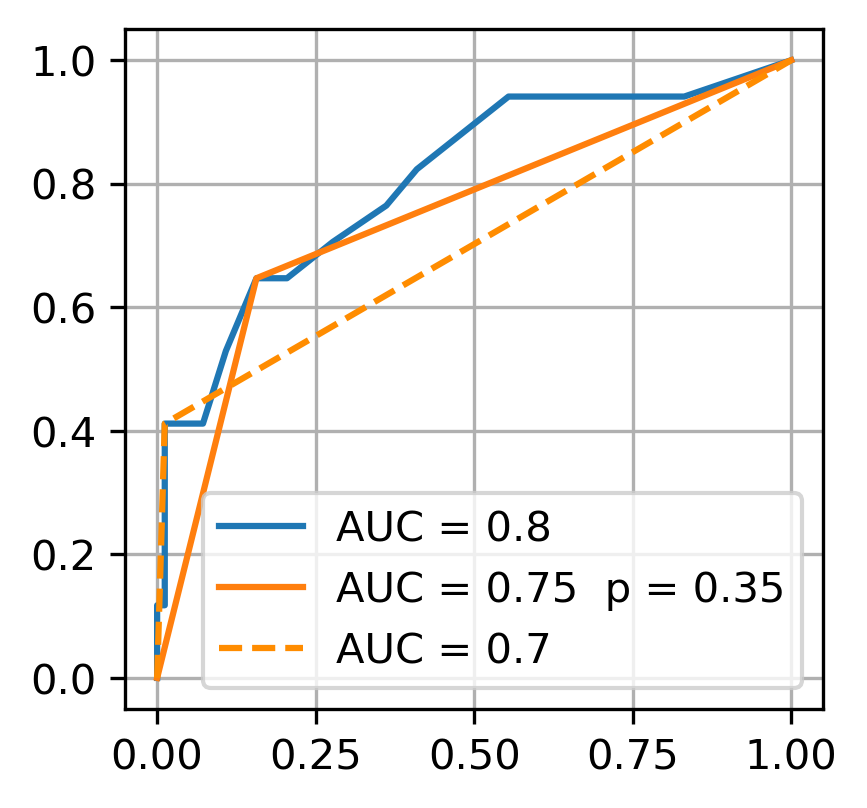
\includegraphics[width=\linewidth]{pictures/Обе метрики при 1 запуске}
		
	\end{minipage}
	\caption{Сравнение метрик  при первом (a) повторном (b) запуске}
\end{figure}
Теперь для вероятностного прогноза метрика AUC равна 0.8, что дает незначительное отклонение от первого запуска. Для бинарного прогноза после бинаризации метрика AUC равна 0.75, и это тоже небольшое отклонение. Для дефолтного бинарного прогноза метрика AUC равна 0.7, то есть, отклонение опять оказывается незначительным. Вместе с тем, порог бинаризации $p$ дает огромное отклонение: при повторном запуске его значение составляет 0.35 вместо бывшего при первом запуске значения 0.15.

\subsection{Сравнение оптимизированного прогноза\\ с дефолтным на множестве запусков}
Чтобы избежать эффекта случайности при разбиении данных, мы производим 250 запусков и усредняем все возникающие при этом показатели так же, как это было сделано на шаге 3.10 (см. рис. 5). Отметим, что, строго говоря, 250 запусков~--- это излишнее количество. Вполне хватило бы и 100. Мы использовали столь больше число только для того, чтобы на графике получилась гладкая ROC-кривая, но если не учитывать визуальную эстетику, меньшее чосло запусков приводит к томуже оптимальному порогу бинаризации.

\begin{figure}[!htb]
	\centering
	\begin{minipage}{0.32\textwidth}
		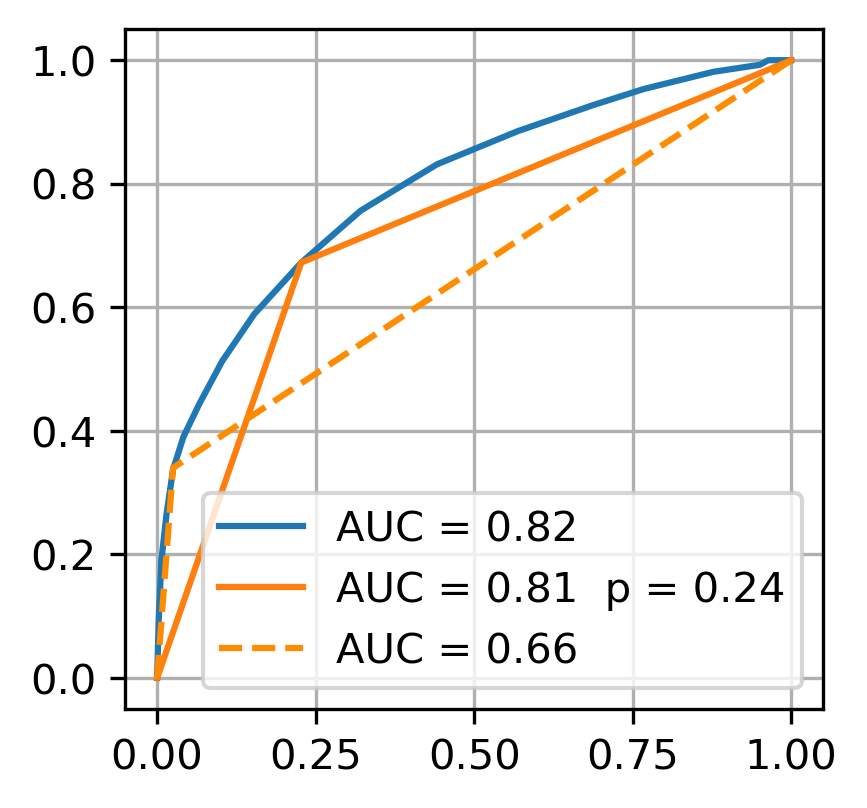
\includegraphics[width=\linewidth]{pictures/Обе метрики на множестве запусков}
	\end{minipage}
	\caption{Обе метрики на множестве запусков}
\end{figure}

При этом стабилизируются все показатели, а самое главное~---  стабилизируется разность между дефолтной и оптимизированной метриками AUC (примерно на уровне $0.81 - 0.66 = 0.15$) и порог бинаризации (примерно на уровне $p = 0.24$).
